%% LyX 2.3.3 created this file.  For more info, see http://www.lyx.org/.
%% Do not edit unless you really know what you are doing.
\documentclass[english]{article}
\usepackage[T1]{fontenc}
\usepackage{float}
\usepackage{amsmath}
\usepackage{graphicx}

\usepackage{subcaption}

\makeatletter

%%%%%%%%%%%%%%%%%%%%%%%%%%%%%% LyX specific LaTeX commands.
%% Because html converters don't know tabularnewline
\providecommand{\tabularnewline}{\\}

\makeatother

\usepackage{babel}
\begin{document}
\title{Project 2}
\author{Zachary Taylor,John Dinofrio, Cristian Bueno}
\maketitle

\part*{Problem 1}

\textbf{Here, we aim to improve the quality of the video sequence provided above. This is a video recording of a highway during night. Most of the Computer Vision pipelines for lane detection or other self-driving tasks require good lighting conditions and color information for detecting good features. A lot of pre-processing is required in such scenarios where lighting conditions are poor. Now, using the techniques taught in class your aim is to enhance the contrast and improve the visual appearance of the video sequence. You can use any in-built functions for the same.}
\bigskip

The provided source video was extremely dark. We resized the image to both speed up our adjustments and make it easier to see the changes side by side with the image source.

\begin{figure}[H]
	\centering
		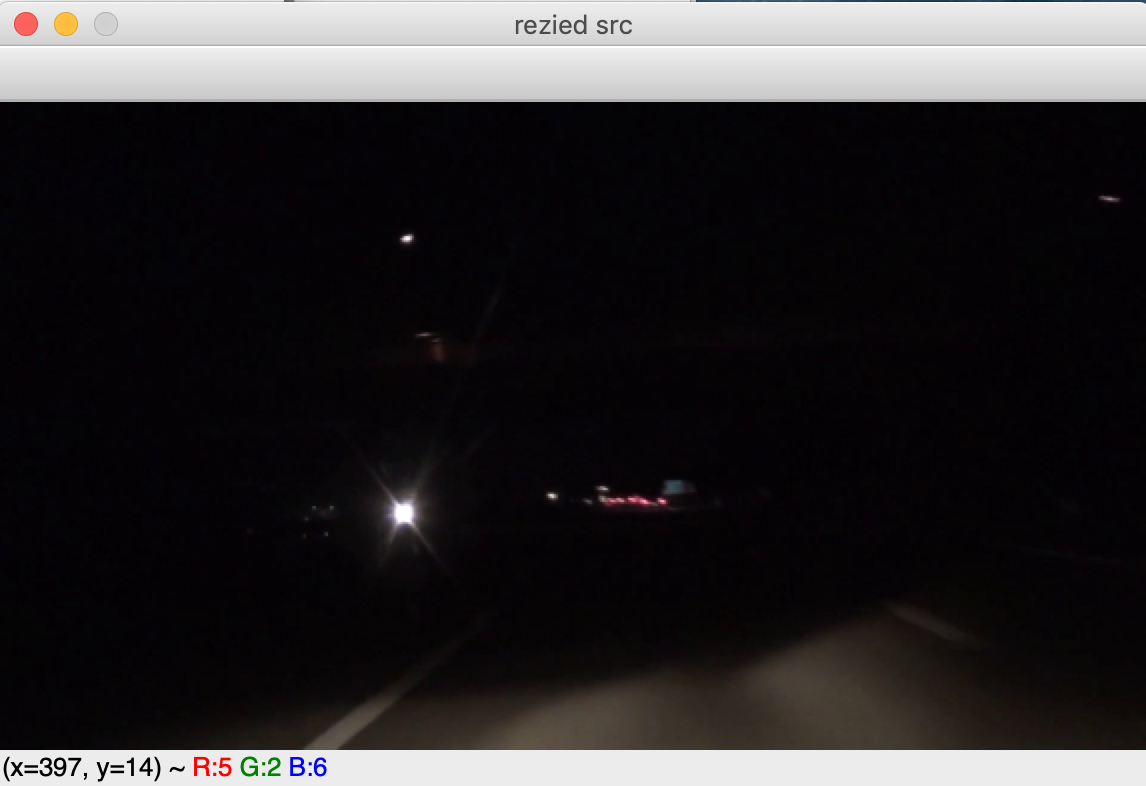
\includegraphics[width = 4in]{./images/src.png}
		\caption{Source Image}
\end{figure}

The first approach we took to solve this problem was using the histogram equalization technique as the effect as demonstrated in the course materials looked powerful. We utilized the built in OpenCV function called equalizeHist() to do this operation. Initially we made each frame grayscale and then equalized, but we also separated the three color channels, equalized each individually, and merged them back together into one image to try to get an equalized color image. We also tried other techniques of converting the image into other color spaces and trying to equalize certain channels that might increase the brightness and contrast, all with little improvement over the other methods. 

\begin{figure}[H]
	\begin{center}
		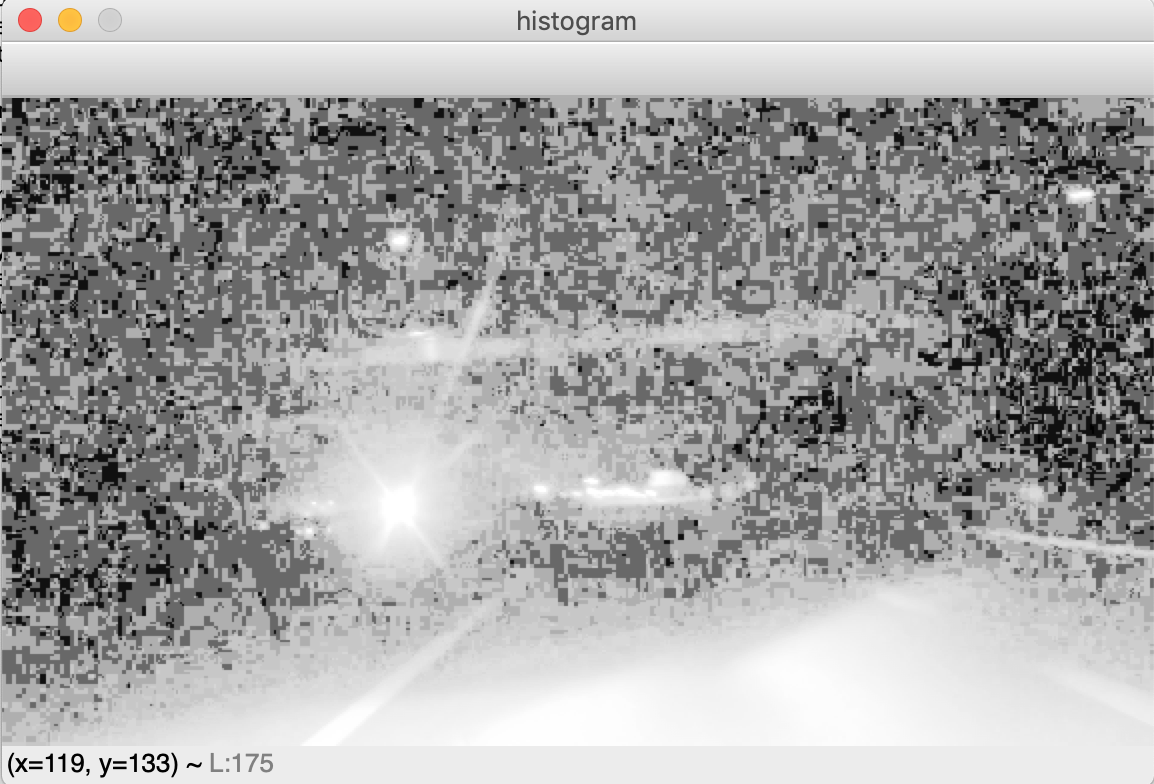
\includegraphics[width = 4in]{./images/gray.png}
	\end{center}
		\caption{Grayscale Histogram Equalization}
\end{figure}
\begin{figure}[H]
	\begin{center}
		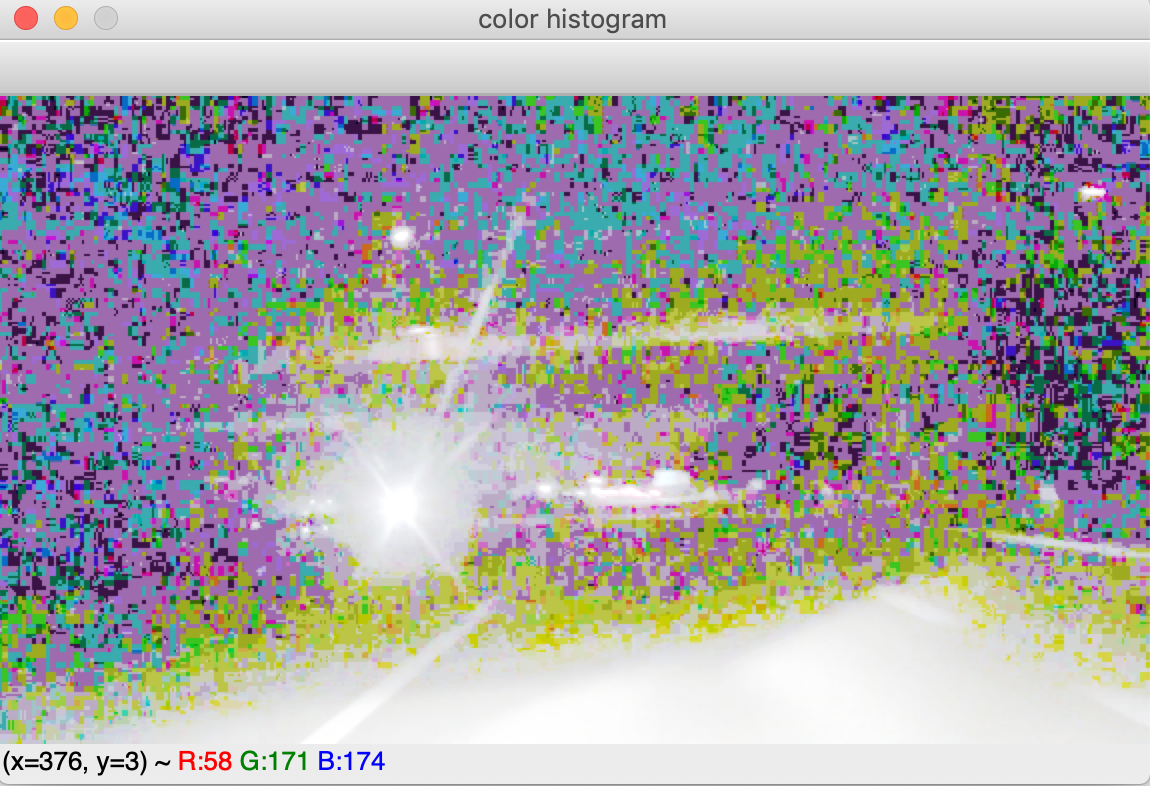
\includegraphics[width = 4in]{./images/color.png}
	\end{center}
		\caption{3 Channel Color Histogram Equalization}
\end{figure}
\begin{figure}[H]
	\begin{center}
		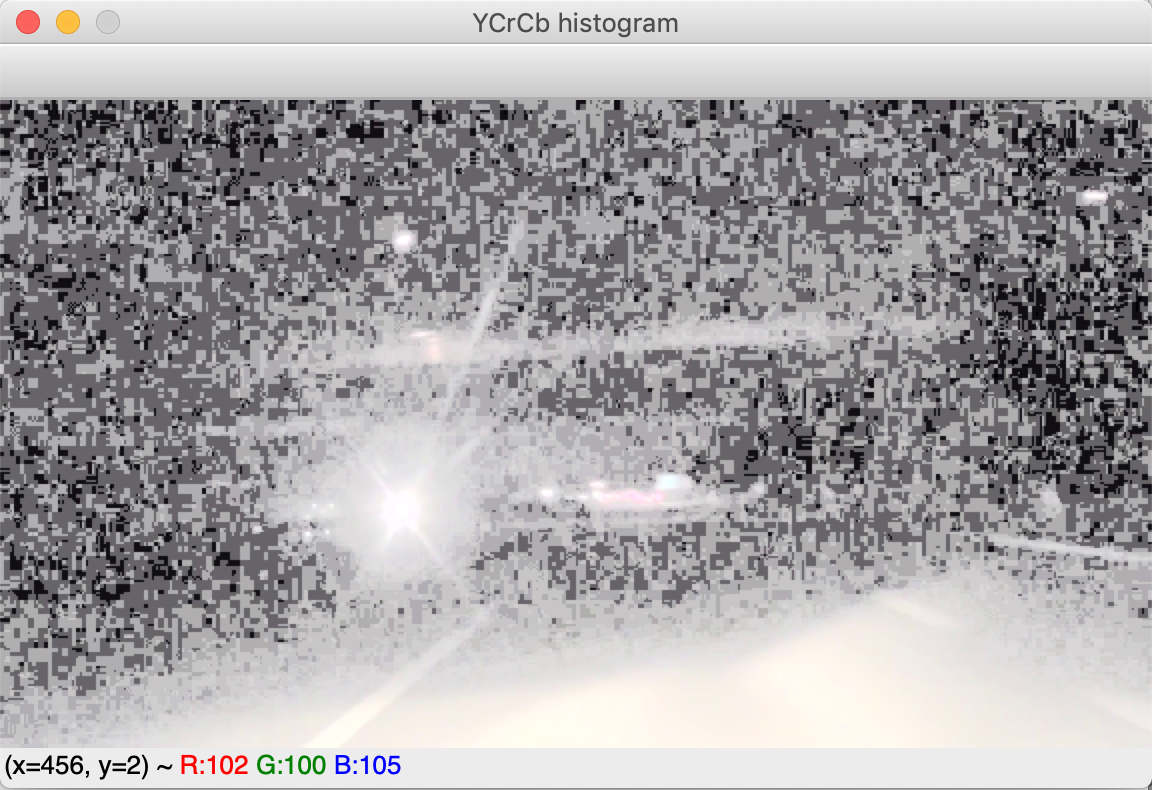
\includegraphics[width = 4in]{./images/yCrCb.png}
	\end{center}
		\caption{YCrCb Histogram Equalization}
\end{figure}

The consistent challenge we had using the built in histogram equalization is that we were getting a lot of noise in the image after equalizing. While it did make it slightly easier to see the lines on the road, the amount of noise in the image may make programmatically finding the lines on the road difficult. We were expecting results similar to what was shown in the class slides that brightened the image and exposed details that otherwise couldn't be seen, but instead got an image with so much noise it was hard to see anything in it. In analyzing the first frame of the video as a sample, we found that the first 25 intensity values on the grayscale image made up 90\% of the pixels in the image. Of those, there were 5 that represented 70\% of the image. Since such a large portion of the image was concentrated in such a narrow range, we can expect some pixelation to occur. This is specifically because each pixel value can only map to one new value, or in other words, we can't add more fidelity to the image than what is already there. That means, since 70\% of our image is populated by only 5 unique values, 70\% of our image, after equalization, will be made up of only 5 different intensity values, just further distributed across the full 8 bit intensity range. This result can be seen clearly by looking at the source and equalized histograms of the image below. Because these values are so spread out, the image looks pixelated instead of smooth. We can do some smoothing after the fact but then some detail is lost in the lane markings we are trying to uncover.

\begin{figure}[H]
	\begin{center}
		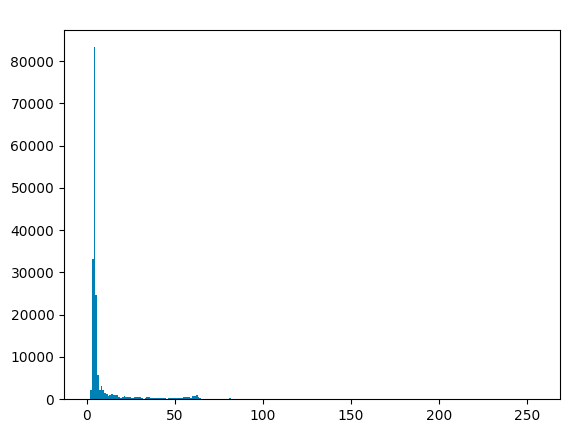
\includegraphics[width = 4in]{./images/grayHist.png}
	\end{center}
		\caption{Source Grayscale Histogram}
\end{figure}
\begin{figure}[H]
	\begin{center}
		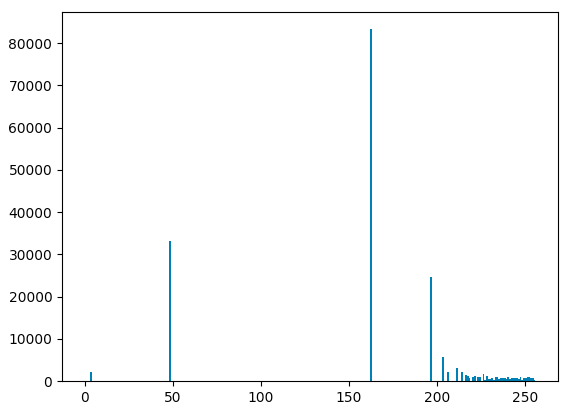
\includegraphics[width = 4in]{./images/grayEqualizedHist.png}
	\end{center}
		\caption{Equalized Histogram}
\end{figure}

Through some research and a desire to do better than what we got with the histogram equalization we were able to find another technique described that adjusts the "gamma" of the image. We found this method ultimately provided the best result of the methods we tested. Instead of trying to equalize the histogram, it maintains the same histogram shape but slides it to the right (increases) on the intensity value. Values starting with a lower intensity slide further to the right than those starting with a higher intensity value, which was also useful in this use case as we didn't want to over expose the light areas like the roads as it could ultimately wash out the lines as well. In effect, this increased the brightness of the overall image but maintains much of the same level of contrast from the source image. We were also able to maintain color correctness using this method as every color channel was adjusted at the same proportion, unlike when we equalized each color channel individually and merged them back together.
\begin{figure}[H]
	\begin{center}
		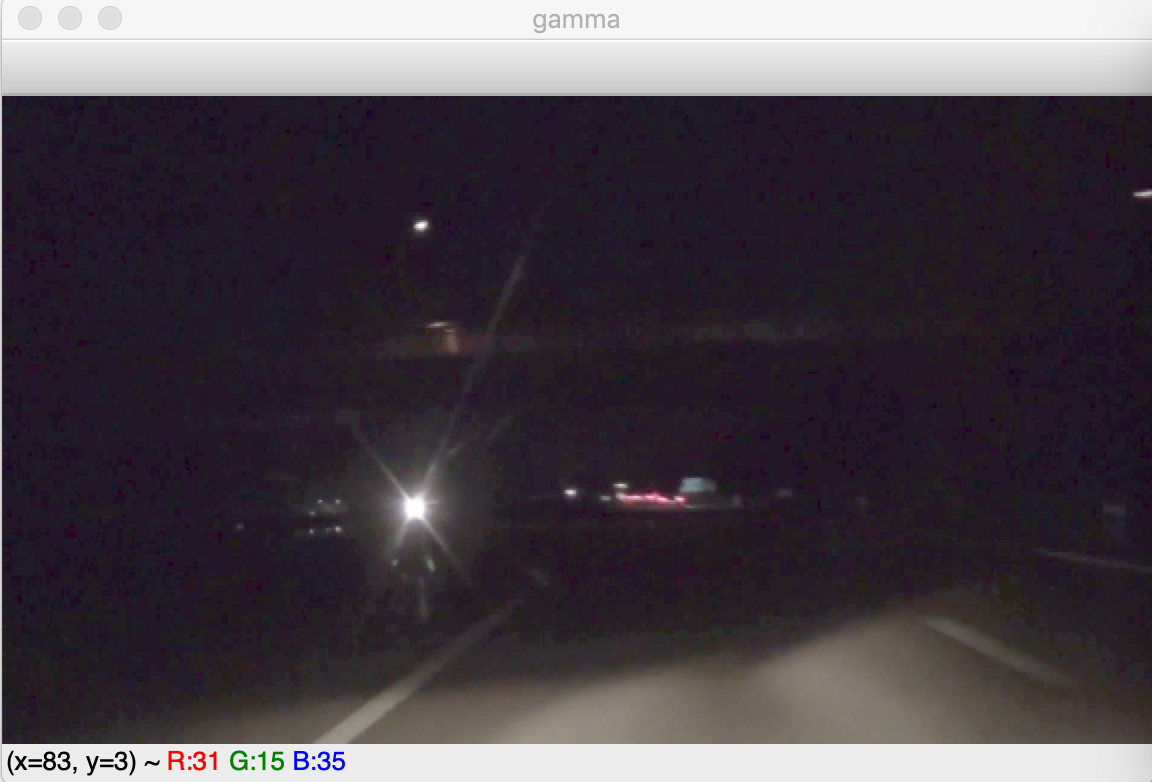
\includegraphics[width = 4in]{./images/gamma.png}
	\end{center}
		\caption{Gamma Adjustment}
\end{figure}
\begin{figure}[H]
	\begin{center}
		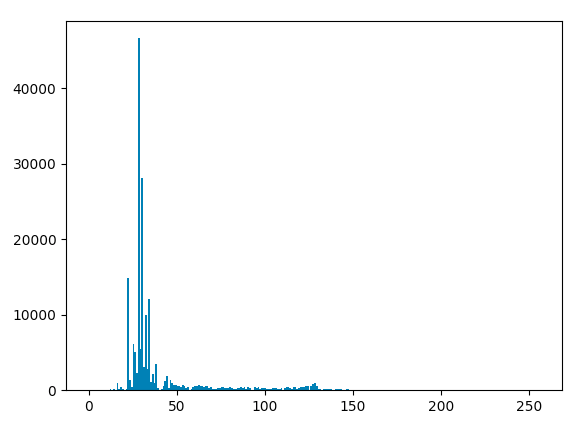
\includegraphics[width = 4in]{./images/gammaHist.png}
	\end{center}
		\caption{Gamma Adjustment Histogram}
\end{figure}
\part*{Problem 2}
\textbf{In this project we aim to do simple Lane Detection to mimic Lane Departure Warning systems used in Self Driving Cars. You are provided with two video sequences (both are required for this assignment), taken from a self driving car (click here to download). Your task will be to design an algorithm to detect lanes on the road, as well as estimate the road curvature to predict car turns.}

In order to detect the lanes and display them as virtual lines on the video, we must correct our camera distortion. 

\begin{figure}[H]
	\begin{center}
		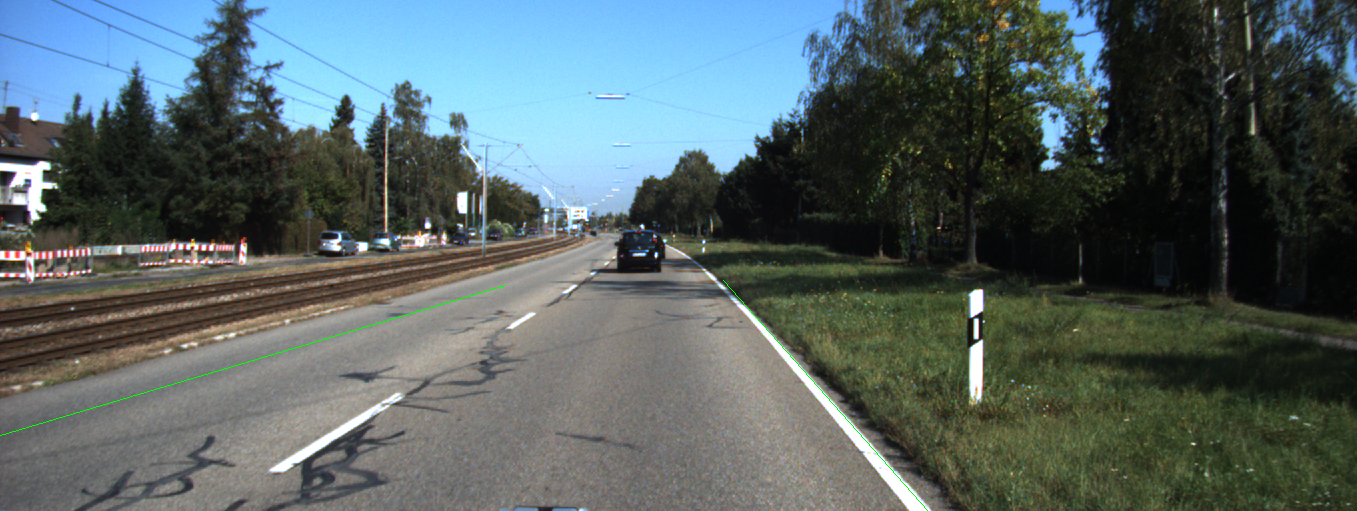
\includegraphics[width = 4in]{./images/Images2/image1.png}
	\end{center}
		\caption{Original frame of the road}
\end{figure}


\begin{figure}[H]
	\begin{center}
		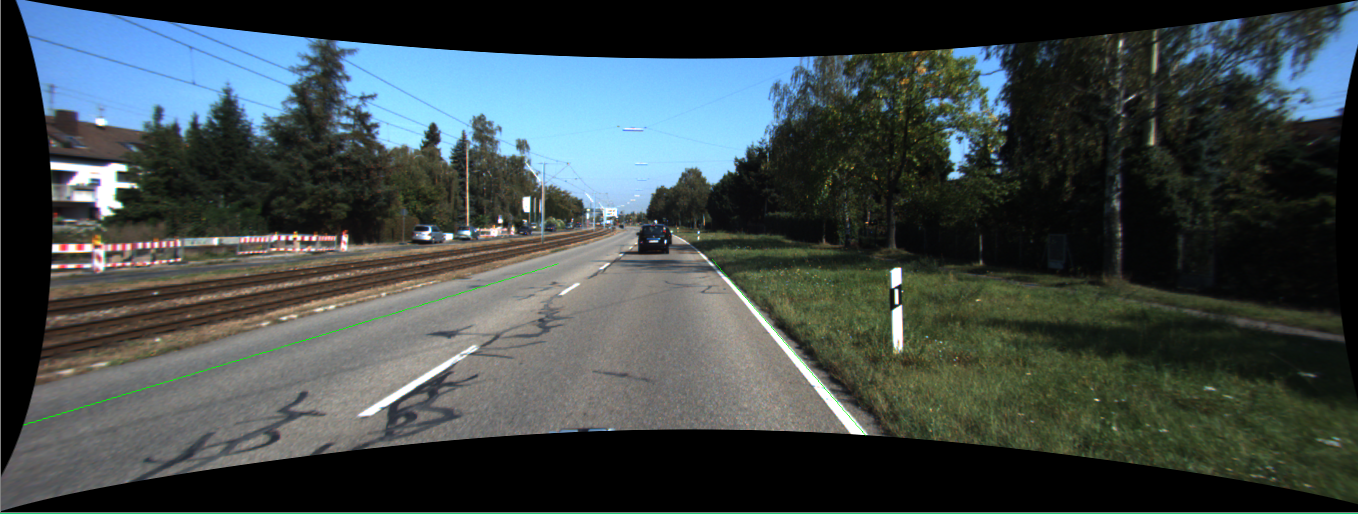
\includegraphics[width = 4in]{./images/Images2/image2.png}
	\end{center}
		\caption{Undistorted frame after K matrix has been applied}
\end{figure}


To find the camera distortion, first, it is necessary to compute the camera matrix. K matrix contains the focal length, and the points of interest of the camera. Distortion coefficients are the values that indicates the sensor of the camera has not parallel lines. 

\begin{equation}
K = \begin{bmatrix}
f_x&0&c_x\\
0&f_y&c_y\\
0&0&1\\
\end{bmatrix};
D=(k_1, k_2, p_1, p_2[, k_3[, k_4, k_5, k_6]])
\end{equation}



After the frame has been corrected, we had to find the homography of the image using four points that we extracted from the road. Using the image with the straightest part of the road, we were able to find four points on the lanes to warp into a top down view. The four points make the visible green lines seen in Figure (10). 

The next step was making the destination points which were any arbitrary points in the shape of a rectangle. With these two sets of 4 points and the OpenCV findHomography function, we created the homography matrix H as well as the inverse homography Matrix H inverse for later use. Then using the built in warp function from OpenCV, we input the image from Figure (10), the H matrix, and the shape of the new image. This gave us Figure (11), the unwarped road.

\begin{figure}[H]
	\begin{center}
		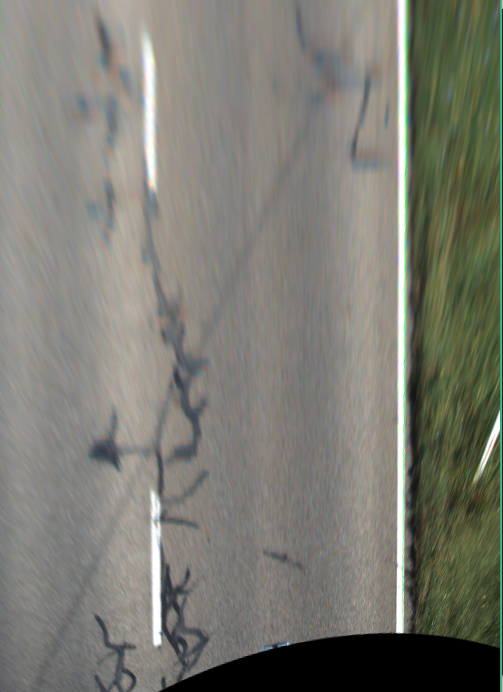
\includegraphics[height = 2in]{./images/Images2/image3.png}
	\end{center}
		\caption{Unwarped image of the road (top down view) after using Homography}
\end{figure}

The next step was thresholding the unwarped road. We found that takinga all pixel values between 210 and 255 gave the best binary image with only the lane lines showing seen in Figure (12). Some objects still made it through, like a couple of road markers and pickets, which caused a problem for us later on.

\begin{figure}[H]
	\begin{center}
		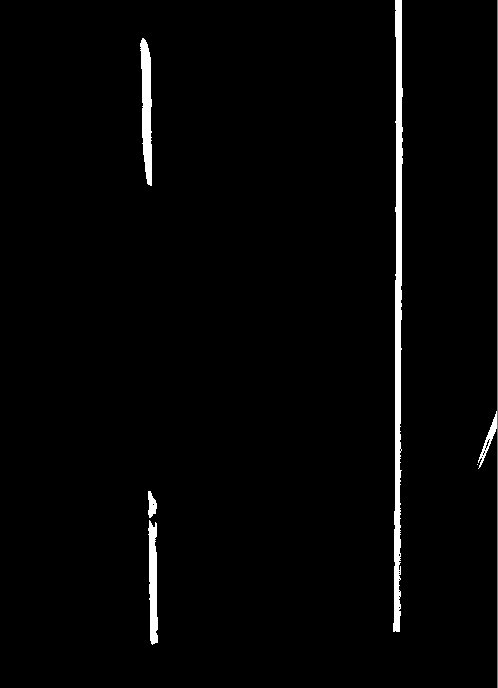
\includegraphics[height = 2in]{./images/Images2/BW_lanes.png}
	\end{center}
		\caption{Binary image of the top down view}
\end{figure}

In order to create the lines, we first have to figure out which parts of the image are the lanes. We used a historgram to do this. Figure (13) shows the histogram of Figure (12) where the x-axis is the width of the image and the y-axis is the total value of pixels in that column.

\begin{figure}[H]
	\begin{center}
		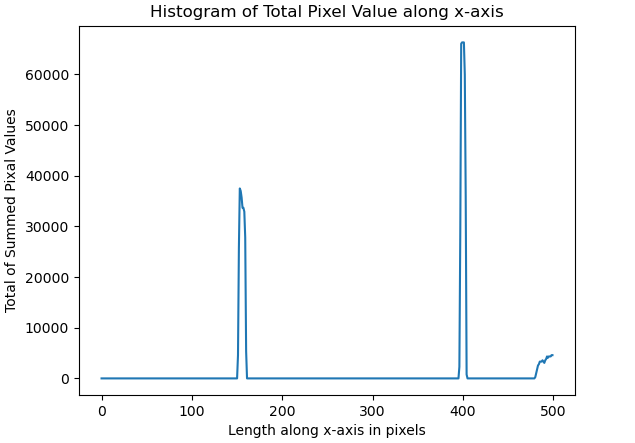
\includegraphics[width = 4in]{./images/Images2/image4.png}
	\end{center}
		\caption{Histogram of the binary top down view of the road}
\end{figure}

Using the regions of the highest pixel concentration, we singled out those areas to be used for edge detection and then least squares fitting.

\begin{figure}[H]
	\begin{center}
		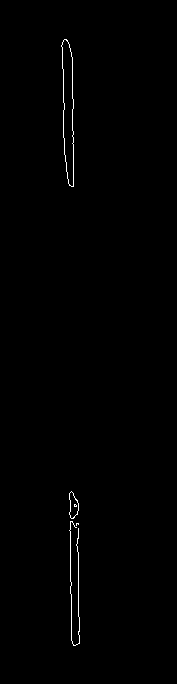
\includegraphics[height = 2in]{./images/Images2/edges.png}
	\end{center}
		\caption{The edges from one lane line}
\end{figure}

The regions selected are then passed through the Canny edge detection funciton from OpenCV. The image is inputted as well as the threshold for how distinct an edge must be to start and continue.

In our application,two different thresholds were defined. One for right lines and left lines, this because the threshold on the right side was detecting unwanted pixels.
\begin{figure}[H]
	\begin{center}
			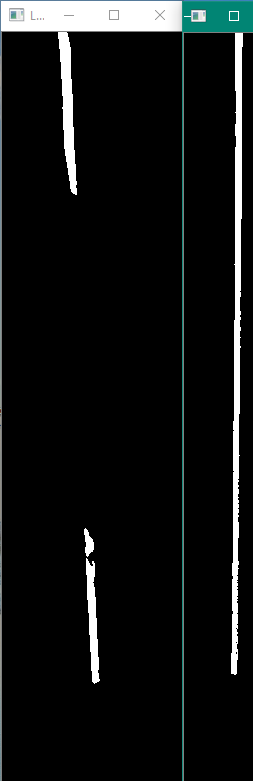
\includegraphics[height=0.5\linewidth]{images/Lines}
	\caption[Right and Left lines]{This lines has different thresholds to avoid unwanted points}
	\label{fig:lines}
	
\end{center}

\end{figure}



Using the findContours OpenCV function on the 
edges, we can find all of the coordinates of the edges. These coordinates can be saved in an array and passed through the least squares fitting function we created. 

In order to find the best curve fit for the lanes, we used least squares line fitting. We switched the x and y coordiantes because we are trying to fit the vertical lines. 

\begin{equation}
X = 
\begin{bmatrix}
x_1\\
x_2\\
\vdots\\
x_{n}\\
\end{bmatrix}
\end{equation}
\begin{equation}
Y = 
\begin{bmatrix}
y^2_1 & y_1 & 1\\
y^2_2 &  y_2 & 1\\
\vdots & \vdots & \vdots\\
y^2_{n} & y_{n} & 1\\
\end{bmatrix}
\end{equation}
\begin{equation}
B = 
\begin{bmatrix}
a\\
b\\
c\\
\end{bmatrix}
\end{equation}

We use linear algebra to find the matrix B so that we can fill in the coefficients for the best curve of fit.

\begin{equation}
x = a * y^2 + b * y + c
\end{equation}

The output of the function is the coefficents of the line fitting function. Using the coefficients, we can use the polyfit function to draw the lanes onto the original top down view of the road. The polyfill function fills in the space between the two lines. Figure (14) shows this.

\begin{figure}[H]
	\begin{center}
		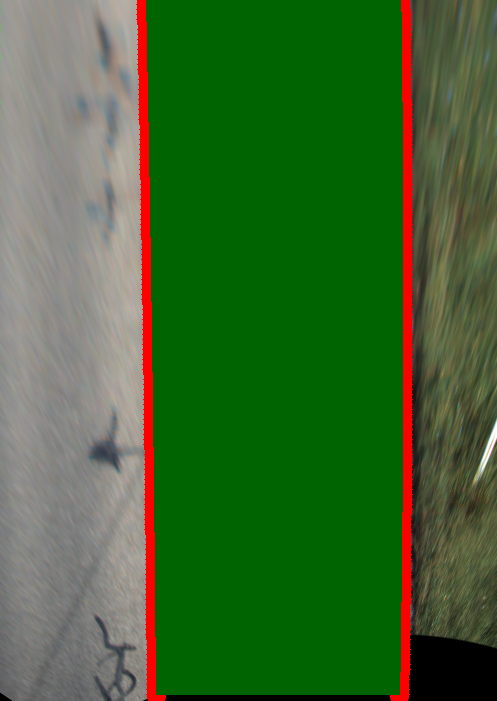
\includegraphics[height = 2in]{./images/Images2/image5.png}
	\end{center}
		\caption{Applying predicted lines and mesh between the lanes to the top down view}
\end{figure}

-----Extra middle line stuff goes here-----


Early in the report we stated that there was difficulty with unwanted objects affecting our program, and the solution to this was simple. Since the road should drastically change curvature within one frame, we created a threshold. If the curveature changed more than the thresholded value, then program was told to use the previous curve parameters. Given more time we could have come up with a more elegant solution that segmented the image better, but this process works well for us.

The next step in the pipeline was putting the superimposed lane back into the orginal undistorted image. This is where the H inverse comes into play. We use the warpPerspective function again with superimposed top down view and the H inverse matrix. This gives us figure (15), a normal perspective view of the road of just the road.

\begin{figure}[H]
	\begin{center}
		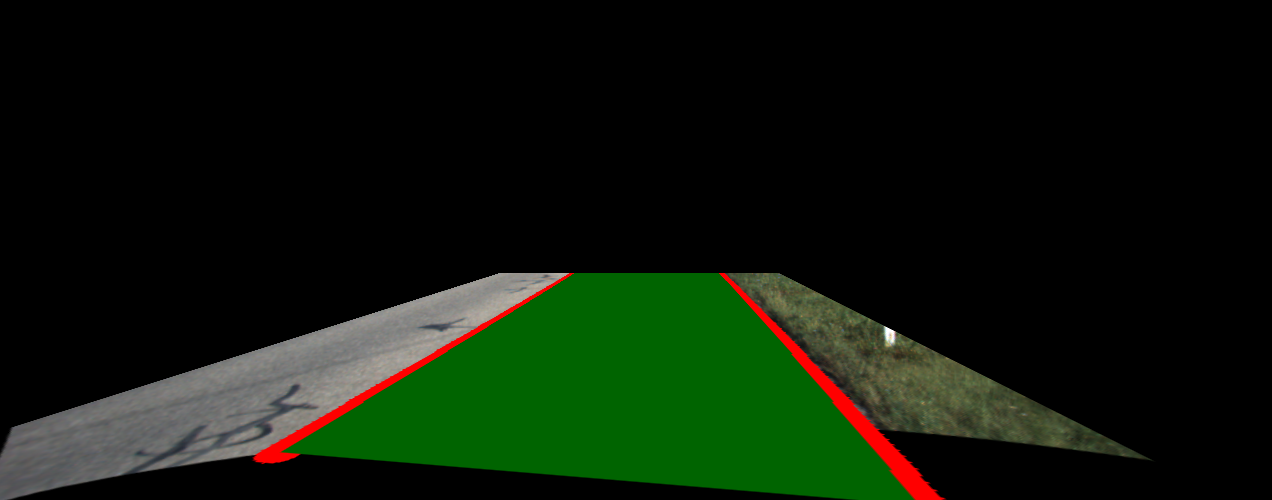
\includegraphics[width = 4in]{./images/Images2/image6.png}
	\end{center}
		\caption{Rewarping the top down view back to the original dimensions}
\end{figure}

The last step is combining the superimposed road with the rest of the image. We used the addWeighted OpenCV function to mix the two images allowing the final image, Figure (16), two look like the normal frame with lines and mesh showing the detected lane.


\begin{figure}[H]
	\begin{center}
		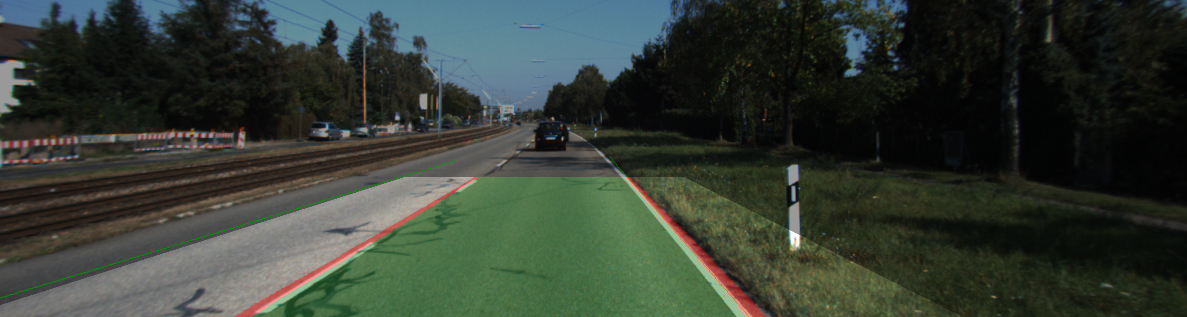
\includegraphics[width = 4in]{./images/Images2/image7.png}
	\end{center}
		\caption{Combinging the original image with the superimposed lanes and mesh}
\end{figure}

To calculate the line that predicts the behavior of the vehicle it was necessary to take the middle point between the new lines detected. So the average of this new points will remain in the center of the road.


\begin{figure}[H]
	\centering
	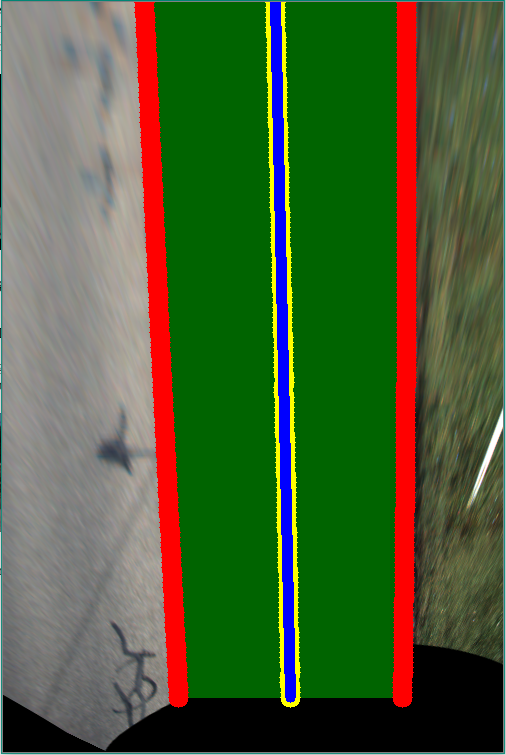
\includegraphics[width=0.7\linewidth]{images/Center}
	\caption[Behavior of the vehicle]{This line shows the guiding line already transformed to an unwarpped position.}
	\label{fig:center}
\end{figure}
After finding this line was necessary to transform back to the original coordinates.
\begin{figure}[H]
	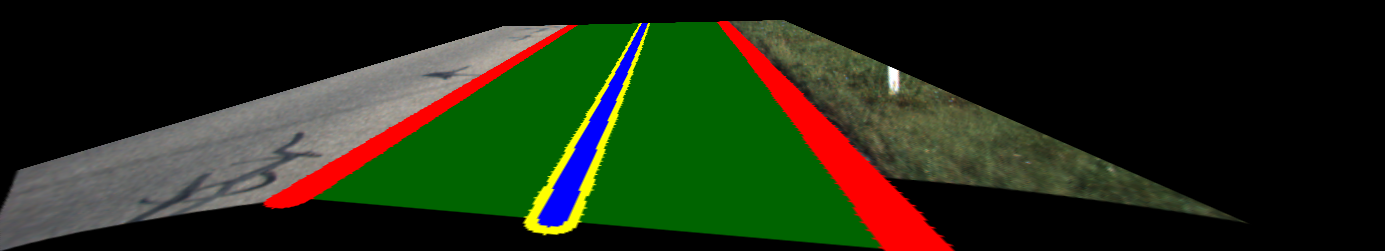
\includegraphics[width=0.9\linewidth]{images/Center2}
	\caption[Line unwarpped]{This figure shows the line projected in the normal space.}
	\label{fig:center2}
\end{figure}

Ones the line that tracks and shows the direction which the vehicle is moving to define were is it moving to a slope equation was used. If the result of this value was negative the car will be moving to the left or if the result of this equation was positive the car will be moving to the right.

\begin{figure}[H]
	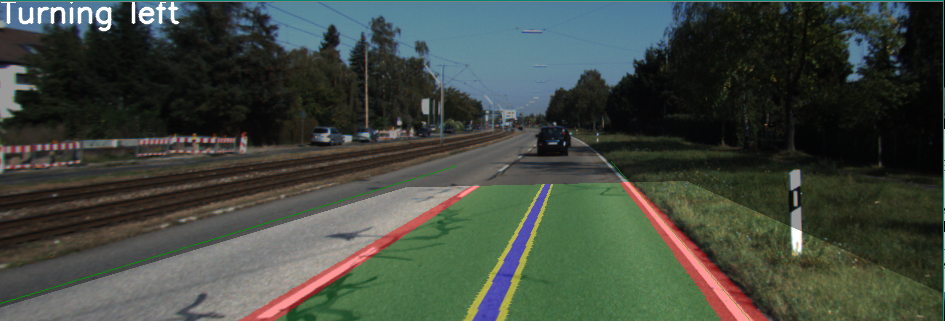
\includegraphics[width=0.9\linewidth]{images/Turning}
	\caption[Turning detection]{This image shows how the algorithm identifies which direction is the car moving to.}
	\label{fig:turning}
\end{figure}
Lastly, to make a better detection on the line slope a kalman filter has been implemented which keep track of the slope and avoid the noise that could exist on the video.
 



 
\end{document}
